\documentclass[a4paper]{article}
\usepackage{amsmath,amssymb}
\usepackage{graphicx} % Required for inserting images
\usepackage{tikz}
\usepackage{hyperref}
\usepackage{cleveref}
\usepackage{pgfplots}
\usetikzlibrary{calc,arrows,shapes,positioning}
\usepackage{standalone}
\usepackage{subcaption}
\usepackage{booktabs}
\usepackage{siunitx} 
\usepackage{IAM_Lager}
\usepackage{float} 

\usepackage[tmargin=0.8cm,lmargin=2cm,rmargin=2cm,bmargin=0.5cm]{geometry}

\newtheorem{problem}{Problem}

\newcommand{\R}{\mathbb{R}}


\title{Maximal moment of a two-span beam}
\author{Michael Gfrerer}
\date{May 2026}

\begin{document}

\maketitle
\begin{abstract}
    In this short note we show that the maximal absolute value of the moment for a two-span beam is at the center support, independently of the span widths.
\end{abstract}
%%%%%%%%%%%%%%%%%%%%%%%%%%%%%%%%%%%%%%%%%%%%%%%%%%%%%%%%%%%%%%
\section*{Proof of the claim}
We consider the two-span beam depicted \Cref{fig:beam}. It is sufficient to consider the moment in the left span for arbitrary $\ell_1$, $\ell_2 > 0$. 
\begin{figure}[H]
    \centering
    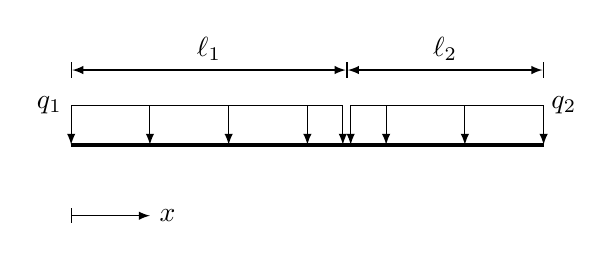
\begin{tikzpicture}[>=latex]
		\coordinate (A) at (0,0);
		\draw[ultra thick] (0,0) -- (6,0);
		\draw[|<->|] (0,0.95) -- ++(3.5,0.0) node[pos=.5,above]{$\ell_1$};
        \draw[|<->|] (3.5,0.95) -- +(2.5,0.0) node[pos=.5,above]{$\ell_2$};
		\foreach \x in {0,1,2,3,3.45,3.55,4,5,6}{
		\draw[<-] (\x,0) -- ++(0,0.5); };
		\draw[] (3.55,0.5) -- (6.0,0.5) node[pos=0.99,right]{$q_2$};
        \draw[] (0,0.5) -- (3.45,0.5)
        node[pos=0.001,left]{$q_1$};
		\Festlager{A};
		\Loslager{3.5,0}[0][1][0];
        \Loslager{6,0};
        \draw[|->] (0,-0.9) -- ++(1,0) node[right]{$x$};
	\end{tikzpicture}	
    \caption{Two-span beam with field lengths $\ell_1$ and $\ell_2$.}
    \label{fig:beam}
\end{figure}
For $0\le x\le \ell_1$ we obtain
\begin{equation}
    M(x) = \frac{x \left(3 \ell_{1}^{3} q_{1} + 4 \ell_{1}^{2} \ell_{2} q_{1} - 4 \ell_{1} q_{1} x \left(\ell_{1} + \ell_{2}\right) - \ell_{2}^{3} q_{2}\right)}{8 \ell_{1} \left(\ell_{1} + \ell_{2}\right)}.
\end{equation}
The maximal moment for the loading $q_1=q$ and $q_2=0$ is 
\begin{equation}
    M_{max}=M(x^*) = \frac{\ell_{1}^{2} q \left(3 \ell_{1} + 4 \ell_{2}\right)^{2}}{128 \left(\ell_{1} + \ell_{2}\right)^{2}}, \quad \text{where}\quad x^*=\frac{\ell_{1} \left(3 \ell_{1} + 4 \ell_{2}\right)}{8 \left(\ell_{1} + \ell_{2}\right)}.
\end{equation}
The minimal moment is obtained at the center support for the loading $q_1=q_2=q$ and reads
\begin{equation}
    M_{min} = -\frac{q \left( \ell_{1}^{2} - \ell_{1} \ell_{2} + \ell_{2}^{2}\right)}{8}.
\end{equation}
We have to show that $M_{max} < |M_{min}|$. For $\ell_1 = a \ell_2$, with $a\in\R_+$ we have
\begin{equation}
    M_{max} + M_{min}  = \frac{\ell_{2}^{2} q \left(a^{2} \left(3 a + 4\right)^{2} + 16 \left(a + 1\right)^{2} \left(- a^{2} + a - 1\right)\right)}{128 \left(a + 1\right)^{2}}.
\end{equation}
Thus, we have $M_{max} < |M_{min}|$ if
\begin{equation}\label{eq::cond}
    f(a) = a^{2} \left(3 a + 4\right)^{2} + 16 \left(a + 1\right)^{2} \left(- a^{2} + a - 1\right) < 0.
\end{equation}
Equivalently, we can show
\begin{equation}\label{eq::cond}
    28 f(a) = -(14a^2-8a-21)^2 -(76a^2+112a+7) < 0.
\end{equation}
For $a\ge0$ we have $-(14a^2-8a-21)^2 \le 0$ and $-(76a^2+112a+7)\le-7$. Therefore, $f(a) \le -\frac{1}{4} < 0$.
\section*{Conclusion}
We have shown that for a two-span beam the maximum of the absolute value of the moment line is
\begin{equation}
    \max_{x}|M(x)| = \frac{q \left( \ell_{1}^{2} - \ell_{1} \ell_{2} + \ell_{2}^{2}\right)}{8}.
\end{equation}


\end{document}
